\chapter{植被冠层和土壤水分}
%\addcontentsline{toc}{chapter}{陆地表面的水分循环}

%\begin{陆地表面的水分循环}
陆地表面的水分循环过程为:
\begin{enumerate}
    \item 降水以液态(雨)或固态(雪)降落到地表,除去被植被截留的部分,其余降落到土壤表面,形成积雪或地面液态水;
    \item 地表液态水可积存在地面,可通过径流方式流走,可入渗到土壤中,或通过蒸发的方式返回大气中;若地表有积雪,积雪中的液态水会由于重力作用自上而下流到土壤表面;
    \item 土壤中的水分会在重力和毛细管力的作用下在土壤孔隙中流动;
    \item 受地势的影响,土壤中的水分会转化为地下径流流走。
\end{enumerate}

对于土壤表面的水分输入,若土壤表面无积雪,则土壤表面水分的输入为
\begin{equation}
G_{water}=P_{ground}+S_{melt}-E
\end{equation}
其中$G_{water}$为到达土壤表面的净水分输入,$P_{ground}$为经植被截留后到达地面的降水,$S_{melt}$为融化的雪水,$E$为土壤表面的蒸发。

若土壤表面有积雪,则考虑水分自上而下到达土壤表面的过程。对最上层积雪,冰的变化量为结霜的量减去升华的量;液态水的增加来自到达雪表面的降水和气态水的凝结,减少的量为蒸发。

积雪中的液态水受毛细管力和重力的共同作用而流动,但由于毛细管力比重力小两个以上数量级,在计算的时候可以忽略。
水流通量一般表达为$K\times{\rm ss}^3$,其中$K$为导水率,$ss$为液态水在孔隙中的饱和度。由于没有有效的参数化方案来计算导水率$K$,
模式中采用简化的方案来近似液态水在积雪中的流动:当某一层中的液态水的含量超过了这一层的持水能力的时候,多余的液态水自这一层流入其下的一层。
最下层的液态水运动,形成对土壤的入渗或地表径流。下面依次从植被到土壤分别介绍各水文循环过程的描述。


\section{植被冠层截留}\label{植被冠层截留}
\begin{mymdframed}{代码}
本节对应的代码文件为\texttt{MOD\_LeafInterception.F90}。
\end{mymdframed}

冠层是降水的首要接触层,它对降水的再分配有着重要的作用。
CoLM支持包括CoLM2014、CLM4.5、CLM5.0、VIC、MATSIRO和Noah-MP等多种冠层截留计算参数化方案。以下针对不同方案分别进行详细介绍。
\subsection{CoLM2014方案}
CoLM冠层的水量平衡方程基本与SiB2一致 \citep{sellers1996revised},主要基于以下控制方程:
\begin{equation}
\partial M_{cw,s}=P-D_{d}-D_{c}-E_{ci} / \rho_{w}
\end{equation}
式中 $P$ 为总降水量(\unit{m.s^{-1}}),分为对流降水和大尺度降水类型:
\begin{equation}
P=P_{c}+P_{l}=\left(R_{c}+S_{c}\right)+\left(R_{l}+S_{l s}\right)
\end{equation}
其中下标$c$和$l$代表对流和大尺度降水类型,$R$和$S$分别代表降雨率与降雪率 (\unit{m.s^{-1}})。
当驱动强迫场中只有总降水可用时,CoLM假设大尺度降水等于$1/3P$,对流降水占$2/3P$。
$D_d$为降雨穿透速率 (\unit{m.s^{-1}}),即从冠层间隙下落的降水速率,$D_c$为冠层排水速度 (\unit{m.s^{-1}}),$\partial M_{cw,s}$为冠层蓄水变化率 (\unit{m.s^{-1}}), 
$\rho_w$是水的密度, $E_{ci}$为蒸发速率。此处的直接穿透量$D_d$与辐射传输中的光穿透量的计算方法一致,由下式给出:
\begin{equation}
D_{d}=\delta_{P} \cdot P=\delta_{P} \cdot\left(R_{c}+S_{c}+R_{l}+S_{l s}\right)
\end{equation}
其中$\delta_P$是冠层穿透系数, 等于
\begin{equation}
\delta_{P}=1.0-\alpha \times\left[1-\exp \left(-K_{p} \times LSAI\right)\right]
\end{equation}
该公式中反映叶片集水能力的经验系数$\alpha$被设定为0.25~\citep{lawrence2011parameterization}。
$LSAI$是$SAI$和$LAI$之和 ($LAI$和$SAI$分别是叶指数和茎面积指数);$K_p$是消光系数,与辐射在冠层中的穿透计算相同:
\begin{equation}\label{Eq:消光系数}
\begin{aligned}
K_{p} &= \phi_{1}+\phi_{2} \\
\phi_{2} &= 0.877\left(1-2 \phi_{1}\right) \\
\phi_{1} &= 0.5-0.633 \chi_{L}-0.33 \chi_{L}^{2}
\end{aligned}
\end{equation}
$K_p$通过叶角分布的经验参数$\chi_L$的变化来控制,
其中$\chi_L=0$表示球形叶角分布,$\chi_L= 1$ 表示水平方向的叶子,$\chi_L= -1$ 表示垂直方向的叶子。
根据植被类型,$\chi_L$的范围在$-0.3\sim0.25$之间。由此计算得出的$\delta_P$的变动范围如图~\ref{fig:穿透系数与叶面积指数} 所示。%
{
\begin{figure}[]
\centering
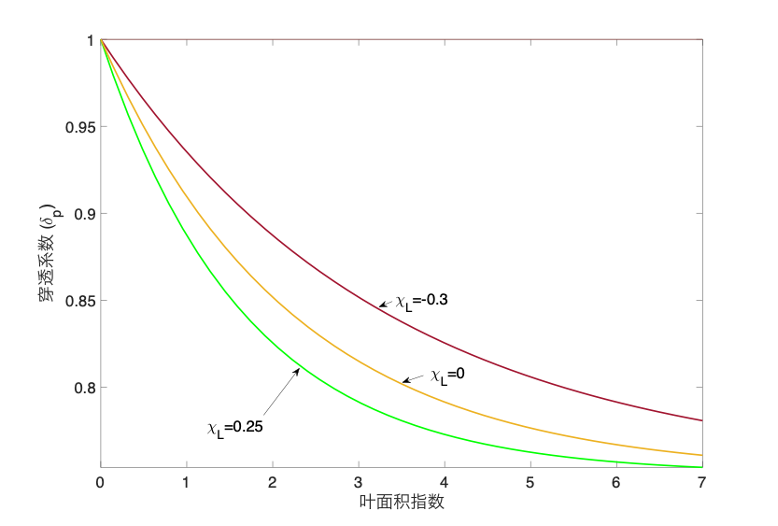
\includegraphics{Figures/陆地表面的水分循环/穿透系数与叶面积指数.png}
\caption{穿透系数$\delta_P$与叶面积指数的关系及其变动范围。}
\label{fig:穿透系数与叶面积指数}
\end{figure}
}

为防止升华或冷凝水超过最大树冠储存量,CoLM在计算冠层截留之前首先更新树叶上的水深 ($L_{dew}$) (mm):
\begin{equation}
\begin{aligned}
L_{dew} &= L_{dew}-x_{sc} \\
x_{s c} &= \max \left(0., L_{dew}-x_{sc}\right)
\end{aligned}
\end{equation}
其中 $x_{sc}$ 是超过最大树冠储存量的水(mm),$S_c=0.1f_{sig}\left(LAI+SAI\right)$代表最大蓄水量(mm)。
$x_{sc}$的相位首先由冠层温度决定。如果冠层温度大于冰点温度,CoLM 假定所有过量的水都处于液相,否则处于冰雪相。

{
\begin{figure}[]
\centering
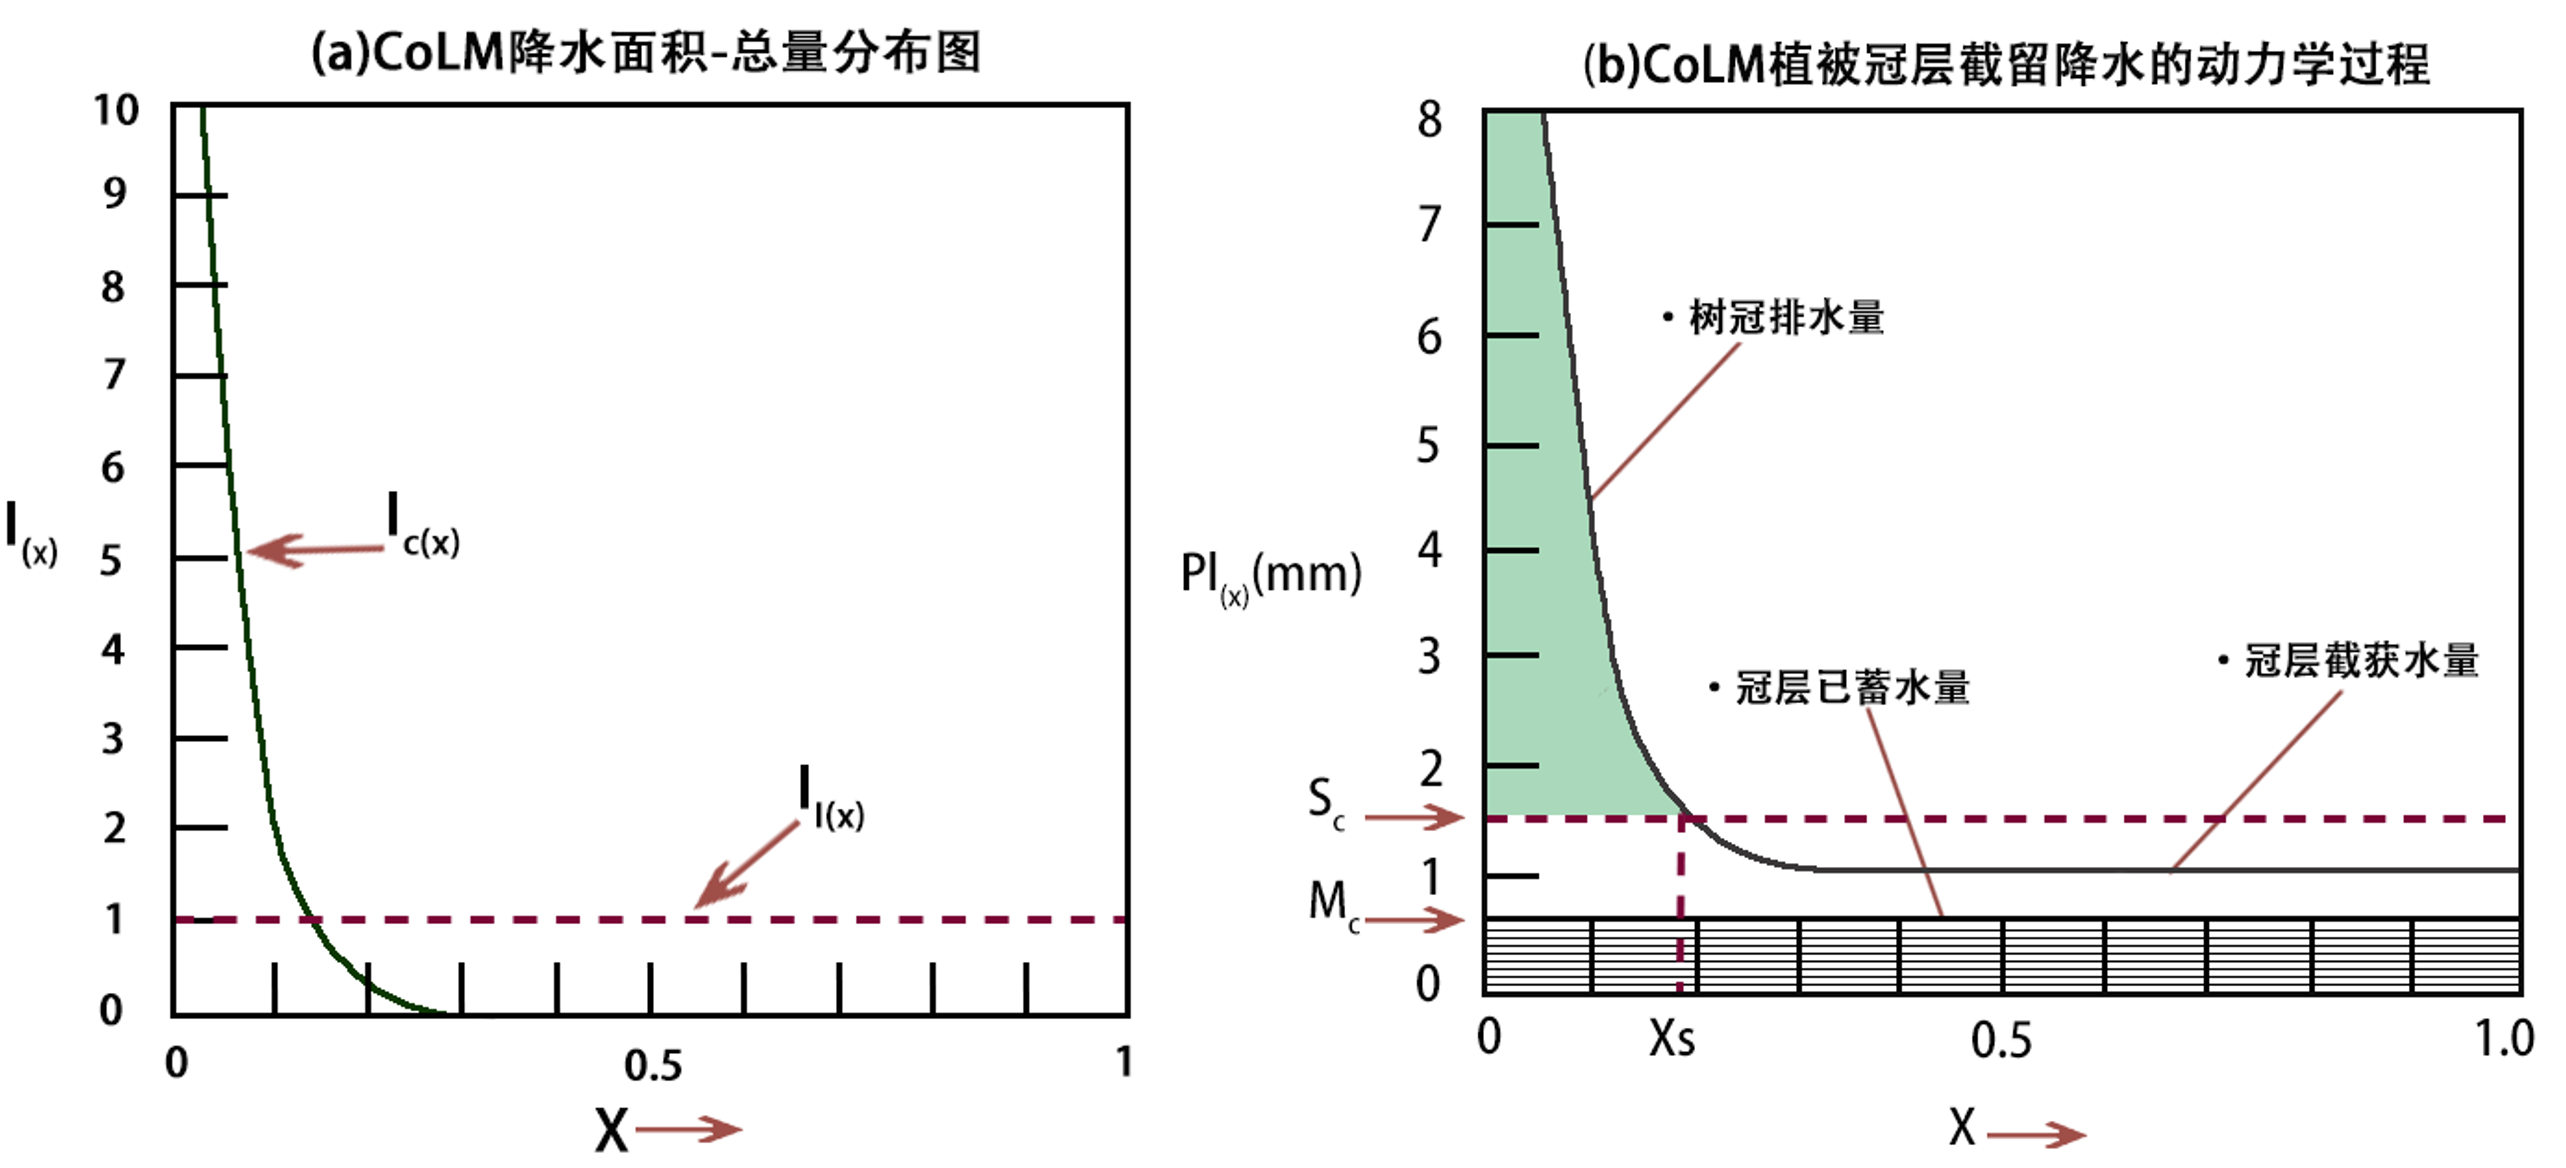
\includegraphics[scale=0.75]{Figures/植被冠层和土壤水分/CoLM冠层截留示意图.png}
\caption{(a) CoLM中使用的降水面积-总量分布图(修改自SiB2。其中变量$x$为网格面积的比例,变量$I_{\left(x\right)}$为相对降水量。值得注意的是,大尺度降水$I_l\left(x\right)$在网格区几乎是不变的,而对流降水$I_c\left(x\right)$是非均匀分布的;(b) CoLM中植被冠层截留降水的动力学过程。降雨截留前已储存在冠层中的水量$M_{cs}-M_{cw}$被假设是均匀分布在网格区域上的。$M_{cs}-M_{cw}$ 的以上的水量积分即为冠层截获的总水量。$xs$是网格区域拦截降雨的比例加上先前存在的树冠蓄水($M_{cs}-M_{cw}$)所超过了树冠最大储水量($S_c$)的水量。所有大于$S_c$的水量假设形成树干径流,而低于$S_c$的水量则被保存在冠层之中。}
\label{fig:CoLM冠层截留示意图}
\end{figure}
}
如图~\ref{fig:CoLM冠层截留示意图}a所示,CoLM 假设网格内的降水的分布是不均匀的。其中对流降水面积的网格占比$I_c$可以由下式给出
\begin{equation}
I_{c}(x)=a_{c} e^{-bx}+c_{c}
\end{equation}
其中$a_c=20$,$b=20$ 和 $c_c=0.206\times10^{-8}$是常数。大尺度降水面积的网格占比$I_l$可以用相同的形式表示:
\begin{equation}
I_{l}(x)=a_{l} e^{-b x}+c_{l}
\end{equation}
其中$a_l=0.0001$和$c_l=0.9999$。因此,通过组合这两个方程给出了有效降雨占比区域的降雨强度为:
\begin{equation}
P I(x)=\left(a_{l} P_{l}+a_{c} P_{c}\right) e^{-b x}+\left(c_{l} P_{l}+c_{c} P_{c}\right)
\end{equation}
如图~\ref{fig:CoLM冠层截留示意图}b所示,因此,有效降雨区域的树冠排水由下式给出:
\begin{equation}
thru_{rain}=\int_{0}^{x_{s}} P I(x) d x+L_{dew} x_{s}-S_{c} x_{s}
\end{equation}
其中$x_s$是单位网格中截获降雨加上原有冠层蓄水量超过冠层上允许的最大水深($S_c$) 的比例:
\begin{equation}
x_{s}=\frac{-1}{b} \log \left[\frac{s_{c}-L_{d e w}}{a_{p}\left(P-D_{d}\right)}-\frac{c_{p}}{a_{p}}\right]
\end{equation}
其中$a_p=\frac{a_lP_l+a_cP_c}{P}$,$c_p=\frac{c_lP_l+c_cP_c}{P}$。这里假设只有液态水能够被冠层所截获,我们有
\begin{equation}
thru_{ {rain }}=\left(R_{c}+R_{l}\right)\left(1-\delta_{p}\right) \frac{a_{p}}{b}\left(1-e^{-b x_{s}}\right)+c_{p} x_{s}+L_{d ew} x_{s}-S_{c} x_{s}
\end{equation}
在整体网格尺度上$D_c$被更新为
\begin{equation}
D_c=thru_{r a i n}+x_{s c}
\end{equation}
因此,保留在树冠上的可用于树冠蒸发(截留蒸发)的蓄水量$I$ (mm)可以由下式进行更新:
\begin{equation}
I={P}-D_{c}-D_{d}
\end{equation}
在冠层蒸发量的计算上首先需要计算湿叶茎面积占总叶茎面积的比例 ($f_{wet}$)。该计算CoLM模型采用~\citet{dickinson1993biosphere}提出的经验方法
\begin{equation}
f_{{wet}}=\left(\frac{L_{dew, p}}{s_{c}}\right)^{2 / 3} \leq 1.0
\end{equation}
其中$L_{dew, p}$是上一步计算得出的可用于树冠蒸发的蓄水量 (m);网格中有效植被的比例为$f_{sig}=\left(1-wt\right)f_{evg}$。
$f_{evg}$是任意网格中植被的比例,$wt$是被雪掩埋的植被占总植被的比例,由下式给出:
\begin{equation}
w t=\frac{0.1 Z_{sno}}{z_{vm}+0.1 Z_{sno}}
\end{equation}
其中$Z_{sno}$代表积雪厚度 (m),$Z_{vm}$代表植被粗糙度 (m)。因此,树冠蒸发量计算如下:
\begin{equation}
E_{ci} / \rho_{w}=\min \left(\frac{\left(q_{s}-q_{sat}^{T_{c}}\right)}{r_{b} /\left(LSAI \times f_{wet}\right)}, \frac{L_{dew}}{\Delta t}\right)
\end{equation}
这里$r_b$是平均边界层阻力,由冠层顶部的风速和特征叶片尺寸确定;$q_{sat}^{T_c}$ (\unit{kg.kg^{-1}}) 是冠层温度下的饱和比湿度;$q_s$为表层参考高度处的比湿度,$\Delta t$为时间步长。

\subsection{CLM4.5模型冠层截留方案}
CLM4.5的冠层截留方案和CoLM2014的方案非常类似。主要的区别在于公式~\eqref{Eq:消光系数} 中的$K_p$的计算。
$K_p$在CLM4.5冠层截留方案中取固定值0.5,即:

\begin{equation}
\delta_{P}=1.0-\alpha \times\left[1-\exp \left(-0.5 \times LSAI\right)\right]
\end{equation}

在原始的CLM4.5方案中并不考虑网格内部的降水类型和分布(假设降水均匀分布在整个网格上),但在现有的方案中遵循CoLM2014的降水分配方案。

\subsection{CLM5.0模型冠层截留方案}
CLM5.0的参数化方案与CLM4.5有较大的差别。其中最重要的差别之一是对雨和雪的截留方案的进一步细化。在CLM5中,液态水的降落过程和CoLM、CLM4.5类似,

\subsection{VIC模型冠层截留方案}

\subsection{MATSIRO模型冠层截留方案}

\subsection{Noah-MP模型冠层截留方案}


\section{土壤水的运动}\label{sec:土壤水的运动}
土壤水的状态和垂直运动主要取决于地表入渗、地下径流、土水势的梯度、重力和植被根部对水的吸收等过程。模式中仅考虑土壤水在垂直方向上的运动。


在非饱和区域,土壤水通量用Buckingham-Darcy定律来描述,
\begin{equation}
q=-K \frac{\partial}{\partial z}(\psi-z)
\end{equation}
其中$z$为土壤深度,取土壤表面为0,垂直向下为正方向,$\psi$为土壤水势,$K$为土壤导水率。


土壤导水率$K$和土水势$\psi$与土壤含水量和土壤质地有关,基于 \citet{clapp1978empirical} 和 \citet{cosby1984statistical} 的工作,
\begin{equation}
\psi=\psi_{s}\left(\frac{\theta}{\theta_{sat}}\right)^{-B}
\end{equation}
\begin{equation}
K=K_{sat}\left(\frac{\theta}{\theta_{sat}}\right)^{2 B+3}
\end{equation}
其中$\psi_s$为饱和土水势,$\theta_{sat}$为饱和土壤体积含水量,$K_{sat}$为饱和导水率,
$\theta$为土壤体积含水量,参数$\psi_s$, $\theta_{sat}$, $K_{sat}$, $B$ 均依赖于土壤质地。


根据质量守恒定律,可得一维土壤水的垂直运动方程(Richards方程),
\begin{equation}
\frac{\partial \theta}{\partial t}=-\frac{\partial q}{\partial z}-Q
\end{equation}
其中$Q$为土壤水的汇,主要为由于根系吸水作用(蒸腾)而减少的水分。


为求解Richards方程,需将土壤在垂直方向分层,
分层方案与计算土壤温度时采用的方案相同。在第$i$层上,对Richards方程进行空间上的积分可得
\begin{equation}
\Delta z_{i} \frac{\partial}{\partial t} \theta_{i}=-\left(q_{i+\frac{1}{2}}-q_{i-\frac{1}{2}}\right)-e_{i}
\end{equation}
\begin{equation}
q_{i+1 / 2}=-K_{i+1 / 2}\left(\frac{\psi_{i+1}-\psi_{i}}{\Delta z_{i}}-1\right)
\end{equation}
其中$\Delta {z_i}$为第$i$层的厚度,$\theta_i$为第$i$层的平均土壤含水量,
$q_{i+\frac{1}{2}}$为第$i$层和第$i+1$层之间的土壤水通量,$q_{i-\frac{1}{2}}$为第$i-1$层和第$i$层之间的土壤水通量,
$e_i$为第$i$层被根系吸收的水分。在时间上采用隐格式,可得
\begin{equation}
\Delta z_{i} \frac{\theta_{i}^{n+1}-\theta_{i}^{n}}{\Delta t}=-\left(q_{i+\frac{1}{2}}^{n+1}-q_{i-\frac{1}{2}}^{n+1}\right)-e_{i}
\end{equation}
\begin{equation}
q_{i+\frac{1}{2}}^{n+1}=-K_{i+\frac{1}{2}}^{n+1}\left(\frac{\psi_{i+1}^{n+1}-\psi_{i}^{n+1}}{\Delta z_{i, i+1}}-1\right)
\end{equation}
其中$\Delta z_{i,i+1}$表示从第$i$层到第$i+1$层中心的距离。
为了简化计算,将$q_{i+\frac{1}{2}}^{n+1}$表达式中的各项在$\theta_i^n$附近做一阶近似,可得
\begin{equation}
\begin{aligned}
K_{i+\frac{1}{2}}^{n+1} &= K_{i+\frac{1}{2}}^{n}+\frac{\partial K_{i+\frac{1}{2}}}
    {\partial \theta_{i}}\left(\theta_{i}^{n+1}-\theta_{i}^{n}\right)+\frac{\partial K_{i+\frac{1}{2}}}
    {\partial \theta_{i+1}}\left(\theta_{i+1}^{n+1}-\theta_{i+1}^{n}\right) \\ 
\psi_{i+1}^{n+1} &= \psi_{i+1}^{n}+\frac{\partial \psi_{i+1}}{\partial \theta_{i+1}}\left(\theta_{i+1}^{n+1}-\theta_{i+1}^{n}\right) \\
\psi_{i}^{n+1} &= \psi_{i}^{n}+\frac{\partial \psi_{i}}{\partial \theta_{i}}\left(\theta_{i}^{n+1}-\theta_{i}^{n}\right)
\end{aligned}
\end{equation}

记$\Delta \theta_i=\theta_i^{n+1}-\theta_i^n$,则
\begin{equation}
\begin{split} 
q_{i+\frac{1}{2}}^{n+1} =&-\left(K_{i+\frac{1}{2}}^{n}+\frac{\partial K_{i+\frac{1}{2}}}{\partial \theta_{i}} \Delta \theta_{i} + \frac{\partial K_{i+\frac{1}{2}}}{\partial \theta_{i+1}} \Delta \theta_{i+1}\right)  \\
    & \times \left(\frac{1}{\Delta z_{i, i+1}}\left(\psi_{i+1}^{n}+\frac{\partial \psi_{i+1}}{\partial \theta_{i+1}} \Delta \theta_{i+1}-\psi_{i}^{n}-\frac{\partial \psi_{i}}
    {\partial \theta_{i}} \Delta \theta_{i}\right)-1\right) \\ 
    \approx & -K_{i+\frac{1}{2}}^{n}\left(\frac{1}{\Delta z_{i, i+1}}\left(\psi_{i+1}^{n}-\psi_{i}^{n}\right)-1\right) \\
    &-\left(-\left(K_{i+\frac{1}{2}}^{n} \frac{1}{\Delta z_{i, i+1}} \frac{\partial \psi_{i}}{\partial \theta_{i}}\right)+\frac{\partial K_{i+\frac{1}{2}}}{\partial 
     \theta_{i}}\left(\frac{1}{\Delta z_{i, i+1}}\left(\psi_{i+1}^{n}-\psi_{i}^{n}\right)-1\right)\right) \Delta \theta_{i} \\ 
    &-\left(\left(K_{i+\frac{1}{2}}^{n} \frac{1}{\Delta z_{i, i+1}} \frac{\partial \psi_{i+1}}{\partial \theta_{i+1}}\right)+\frac{\partial K_{i+\frac{1}{2}}}{\partial
      \theta_{i+1}}\left(\frac{1}{\Delta z_{i, i+1}}\left(\psi_{i+1}^{n}-\psi_{i}^{n}\right)-1\right)\right) \Delta \theta_{i+1} 
\end{split}
\end{equation}
对$q_{i-\frac{1}{2}}^{n+1}$也可做同样的近似。从而,完全离散后的Richards方程可表达为,
\begin{equation}
{a}_{{mx}} \Delta \theta_{i-1}+b_{m x} \Delta \theta_{i}+c_{m x} \Delta \theta_{i+1}=r_{m x}
\end{equation}
其中,
\begin{equation}
\begin{aligned}
 a_{mx} &= -\left(K_{i-\frac{1}{2}}^{n} \frac{1}{\Delta z_{i-1, i}}
     \frac{\partial \psi_{i-1}}{\partial \theta_{i-1}}\right)+\frac{\partial K_{i-\frac{1}{2}}}
     {\partial \theta_{i-1}}\left(\frac{1}{\Delta z_{i-1, i}}\left(\psi_{i}^{n}-\psi_{i-1}^{n}\right)-1\right) \\
b_{mx} &= \frac{\Delta z_{i}}{\Delta t}-\left(-\left(K_{i+\frac{1}{2}}^{n} \frac{1}{\Delta z_{i, i+1}} 
      \frac{\partial \psi_{i}}{\partial \theta_{i}}\right)+\frac{\partial K_{i+\frac{1}{2}}}{\partial \theta_{i}}
      \left(\frac{1}{\Delta z_{i, i+1}}\left(\psi_{i+1}^{n}-\psi_{i}^{n}\right)-1\right)\right) \\
&\mathrel{\phantom{=}}+\left(\left(K_{i-\frac{1}{2}}^{n} \frac{1}{\Delta z_{i-1, i}} \frac{\partial \psi_{i}}{\partial 
       \theta_{i}}\right)+\frac{\partial K_{i-\frac{1}{2}}}{\partial \theta_{i}}\left(\frac{1}{\Delta z_{i-1, i}}\left(\psi_{i}^{n}-\psi_{i-1}^{n}\right)-1\right)\right) \\ 
c_{mx} &= -\left(\left(K_{i+\frac{1}{2}}^{n} \frac{1}{\Delta z_{i, i+1}} 
       \frac{\partial \psi_{i+1}}{\partial \theta_{i+1}}\right)+\frac{\partial K_{i+\frac{1}{2}}}{\partial \theta_{i+1}}\left(\frac{1}
       {\Delta z_{i, i+1}}\left(\psi_{i+1}^{n}-\psi_{i}^{n}\right)-1\right)\right) \\ 
r_{mx} &= K_{i+\frac{1}{2}}^{n}
       \left(\frac{1}{\Delta z}\left(\psi_{i+1}^{n}-\psi_{i}^{n}\right)+1\right)-K_{i-\frac{1}{2}}^{n}
       \left(\frac{1}{\Delta z}\left(\psi_{i}^{n}-\psi_{i-1}^{n}\right)-1\right)-e_{i}
\end{aligned}
\end{equation}

对最上面的土壤分层(第1层),使用给定的入渗通量$q_{infl}$,则
\begin{equation}
\begin{aligned}
a_{mx} &= 0 \\
b_{mx} &= \frac{\Delta z_{i}}{\Delta t}-\left(-\left(K_{i+\frac{1}{2}}^{n} 
    \frac{1}{\Delta z_{i, i+1}} \frac{\partial \psi_{i}}{\partial \theta_{i}}\right)+\frac{\partial K_{i+\frac{1}{2}}}{\partial \theta_{i}}\left(\frac{1}{\Delta z_{i, i+1}}
    \left(\psi_{i+1}^{n}-\psi_{i}^{n}\right)-1\right)\right) \\
c_{mx} &= -\left(\left(K_{i+\frac{1}{2}}^{n} \frac{1}{\Delta z_{i, i+1}} 
    \frac{\partial \psi_{i+1}}{\partial \theta_{i+1}}\right)+\frac{\partial K_{i+\frac{1}{2}}}{\partial \theta_{i+1}}\left(\frac{1}{\Delta z_{i, i+1}}
    \left(\psi_{i+1}^{n}-\psi_{i}^{n}\right)-1\right)\right) \\ 
r_{mx} &= q_{i n f l}+K_{i+\frac{1}{2}}^{n}
    \left(\frac{1}{\Delta z}\left(\psi_{i+1}^{n}-\psi_{i}^{n}\right)-1\right)-e_{i}
\end{aligned}
\end{equation}
对最下面的土壤分层,假定边界条件为重力排水边界条件,即$q_{i+\frac{1}{2}}^{n+1}=-K_{i+\frac{1}{2}}^{n+1}$,则
\begin{equation}
\begin{aligned}
a_{mx} &= -\left(K_{i-\frac{1}{2}}^{n} \frac{1}{\Delta z_{i-1, i}} \frac{\partial \psi_{i-1}}
    {\partial \theta_{i-1}}\right)+\frac{\partial K_{i-\frac{1}{2}}}{\partial \theta_{i-1}}\left(\frac{1}{\Delta z_{i-1, i}}
    \left(\psi_{i}^{n}-\psi_{i-1}^{n}\right)-1\right) \\
b_{mx} &= \frac{\Delta z_{i}}{\Delta t}+\frac{\partial K_{i+\frac{1}{2}}}
    {\partial \theta_{i}}+\left(\left(K_{i-\frac{1}{2}}^{n} \frac{1}{\Delta z_{i-1, i}} \frac{\partial \psi_{i}}{\partial \theta_{i}}\right)+
    \frac{\partial K_{i-\frac{1}{2}}}{\partial \theta_{i}}\left(\frac{1}{\Delta z_{i-1, i}}\left(\psi_{i}^{n}-\psi_{i-1}^{n}\right)-1\right)\right) \\
c_{mx} &= 0 \\
r_{mx} &= -K_{i+\frac{1}{2}}^{n}-K_{i-\frac{1}{2}}^{n}\left(\frac{1}{\Delta z}\left(\psi_{i}^{n}-\psi_{i-1}^{n}\right)-1\right)-e_{i}
\end{aligned}
\end{equation}
求解上述方程组,即可得到土壤水含量的变化量。方程组的系数矩阵为三对角阵,可用追赶法快速求解。


在系数矩阵中,需要对土水势和导水率函数求导数。对土水势,容易计算得到
\begin{equation}
\frac{\partial \psi_{i}}{\partial \theta_{i}}=-B \frac{\psi_{i}}{\theta_{i}}
\end{equation}
对导水率,若采用迎风格式
\begin{equation}
    K_{i+1/2}=\left\{\begin{array}{rl} K_{ {sat }}\left(\frac{\theta_{i}}{\theta_{ {sat }}}\right)^{2 B+3},
       & -\left(\frac{\psi_{i+1}-\psi_{i}}{\Delta z}-1\right) \geq 0 \\ K_{ {sat }}\left(\frac{\theta_{i+1}}{\theta_{ {sat }}}\right)^{2 B+3},
       & -\left(\frac{\psi_{i+1}-\psi_{i}}{\Delta z}-1\right)<0\end{array}\right.
\end{equation}
则导数为
\begin{equation}
\frac{\partial K_{i+\frac{1}{2}}}{\partial \theta_{i}}=\begin{cases}
  (2 B+3) K_{ {sat }}\left(\frac{\theta_{i}}{\theta_{sat}}\right)^{2 B+2} 
    \frac{1}{\theta_{s a}}, & -\left(\frac{\psi_{i+1}-\psi_{i}}{\Delta z}-1\right) \geq 0 \\ 
   0, & -\left(\frac{\psi_{i+1}-\psi_{i}}{\Delta z}-1\right) < 0 
  \end{cases}
\end{equation}
\begin{equation}
\frac{\partial K_{i+\frac{1}{2}}}{\partial \theta_{i+1}}=\begin{cases}
     0, & -\left(\frac{\psi_{i+1}-\psi_{i}}{\Delta z}-1\right) \geq 0 \\
     (2 B+3) K_{ {sat }}\left(\frac{\theta_{i+1}}{\theta_{ {sat }}}\right)^{2 B+2} \frac{1}{\theta_{ {sat }}}, & -\left(\frac{\psi_{i+1}-\psi_{i}}{\Delta z}-1\right) <0 
   \end{cases}
\end{equation}
对计算区域的底部,
\begin{equation}
K_{i+1 / 2}=K_{ {sat }}\left(\frac{\theta_{i}}{\theta_{ {sat }}}\right)^{2 B+3}, \quad \frac{\partial K_{i+\frac{1}{2}}}
{\partial \theta_{i}}=(2 B+3) K_{ {sat }}\left(\frac{\theta_{i}}{\theta_{ {sat }}}\right)^{2 B+2} \frac{1}{\theta_{sat}}
\end{equation}
有冰存在的时候,需考虑冰对导水率的影响,使用如下经验公式,
\begin{equation}
    {f}_{{imped}, {i}+1 / 2}=10^{-e_{ice}\times 0.5\times\left(f_{i c e, i}+f_{i c e, i+1}\right)}
\end{equation}
其中$e_{ice}=6.0$为冰的阻抗因子。对导水率及其导数的调整为
\begin{equation}
\begin{array}{c}K_{i+\frac{1}{2}}={f}_{ {imped,i+ }+\frac{1}{2}} \times K_{i+\frac{1}{2}} \\ \frac{\partial K_{i+\frac{1}{2}}}{\partial \theta_{i}}
    ={f}_{ {imped,i+ }+\frac{1}{2}} \times \frac{\partial K_{i+\frac{1}{2}}}{\partial \theta_{i}} \\ \frac{\partial K_{i+\frac{1}{2}}}{\partial \theta_{i+1}}=
    {f}_{ {imped,i+ } \frac{1}{2}} \times \frac{\partial K_{i+\frac{1}{2}}}{\partial \theta_{i+1}}\end{array}
\end{equation}


对地下水的补给率定义为最下层土壤流出的水流通量,
\begin{equation}
{q}_{ {charge }}=q_{I+\frac{1}{2}}^{n+1}=K_{I+\frac{1}{2}}^{n}+\frac{\partial K_{I+\frac{1}{2}}}{\partial \theta_{I}} \Delta \theta_{I}
\end{equation}


这里对土壤水方程中的源汇项$Q$的主要来源,即根系吸水作用(蒸腾)过程做一简单介绍。植物吸水作用由有效根比例$f_{root,i}$和叶面蒸腾$E_{tr}$的乘积来表示\citep{dai2003common}。有效根比例为:
\begin{equation}
{f}_{ {root }, {i}}=\frac{{f}_{{root}, {i}} {W}_{{LT}}[{i}]}{W_{t}}
\end{equation}
其中$Wt = \sum_{i=1}^{n}{f_{root,i\ }W_{LT}\left[i\right]}$;$f_{root,i}$表示模式中第$i$层土壤中的根系比例;$W_{LT}[i]$表示第$i$层土壤中的水分胁迫状况:
\begin{equation}
{W}_{{LT}}[{i}]=\frac{\psi_{\max }-\psi_{i}}{\psi_{\max }-\psi_{sat}}
\end{equation}
其中,$\psi_{max}$为植物叶片干枯前的最大水势。


叶面蒸腾表示为:
\begin{equation}
{E}_{{tr}}=\sigma_{{f}} LSAI \delta\left({E}_{{f}}^{{pot}}\right) {L}_{{d}} \frac{{r}_{{b}}}{{r}_{{b}}-{r}_{{s}}} {E}_{{f}}^{{pot}} \leq {E}_{{trmax}}
\end{equation}
其中,$\sigma_f$表示没有被雪覆盖的植物比例,$LSAI$表示叶面积指数和茎面积指数之和,$\delta\left(E_f^{pot}\right)$为表示蒸发是否发生的参数,
取值0或1,$L_d$为干燥的植物表面比例,$r_b$为叶片边界层阻抗,$r_s$为叶片气孔阻抗。$E_f^{pot}$表示植物表面水的单位面积蒸发量:
\begin{equation}
{E}_{{f}}^{{pot}}=\rho_{{a}} {r}_{{b}}^{-1}\left({q}_{{f}}^{{sat}}-{q}_{{af}}\right)
\end{equation}
其中,$\rho_a$表示空气密度,$q_f^{sat}$表示冠层空气饱和比湿,$q_{af}$表示冠层空气比湿。$E_{trmax}$为最大蒸腾速率:
\begin{equation}
{E}_{ {trmax }}=2 \times 10^{-4} \times \sigma_{{f}} L A I \times W_{t}
\end{equation}
\section{地下水与土壤水的相互作用}
地下水的运动包含土壤水对地下水的补给和由地形起伏引起的地下径流。


给水度(specific yield)反映了地下水位变化时土壤水的变化量。模式中采用分析公式来计算,
\begin{equation}
{S}_{{y}}=\theta_{s}\left(1-\left(1-\frac{z_{w t}}{\psi_{s}}\right)^{-1 / b}\right)
\end{equation}
含水层水量的变化为
\begin{equation}
w_{a}=w_{a}+q_{charge} \times \Delta t
\end{equation}
若地下水位位于最下层土壤之下,则水位的变化为
\begin{equation}
Z_{w t}=z_{w t}-\frac{q_{charge} \times \Delta t}{s_{y}}
\end{equation}
若地下水位位于分层土壤之内,则需要逐层计算水位的变化。当$q_{charge}>0$时,
由地下水位所在一层开始,至最上层或补给水用尽结束,依次计算,
\begin{equation}
\begin{array}{c}{S}_{{y}}=\theta_{s}\left(1-\left(1-\frac{z_{w t}}{\psi_{s}}\right)^{-1 / b}\right) \\
     q_{ {charge }, i}=\min \left(q_{ {charge }}, S_{y} \times \left(z_{w t}-z_{i-1, i}\right)\right) \\
      q_{ {charge }}=q_{ {charge }}-q_{ {charge }, i} \\ 
      z_{w t}=\max \left(0, z_{w t}-q_{ {charge }, i} / S_{y}\right)\end{array}
\end{equation}

\section{可变饱和流数值算法}
可变饱和流数值算法将地表入渗、土壤水运动和土壤水与地下水的相互交换这三个垂直方向的水流运动进行统一求解(图 \ref{fig:可变饱和流数值算法预报区域空间结构示意图})。
{
\begin{figure}[]
\centering
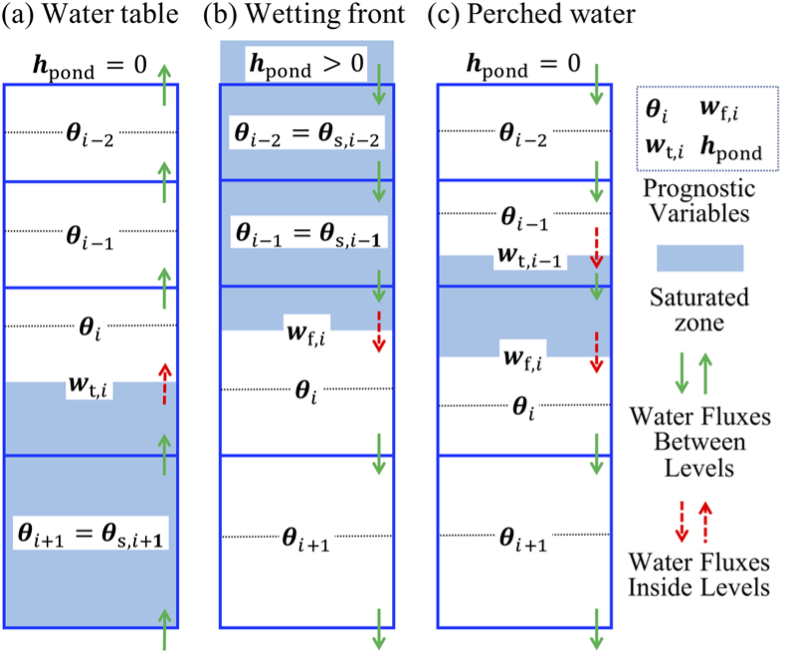
\includegraphics{Figures/陆地表面的水分循环/可变饱和流数值算法预报区域空间结构示意图.png}
\caption{可变饱和流数值算法预报区域空间结构示意图。}
\label{fig:可变饱和流数值算法预报区域空间结构示意图}
\end{figure}
}

\subsection{土壤水预报方程}
在每个土壤层内,有三个预报变量来描述土壤中液态水的分布情况。
土壤体积含水量为固定的预报变量($\theta_i$)。为了追踪土壤中饱和水层的变化(包括地下水、滞水层和入渗情况下由地表向下发展的饱和水层),
每层土壤中引入了另外两个潜在的预报变量($w_{f,i}$和$w_{t,i}$),
分别代表土壤层内上部饱和区域的厚度,和土壤层内下部饱和区域的厚度(图~\ref{fig:可变饱和流数值算法预报区域空间结构示意图}),
当某层土壤部分饱和时,这两个变量被激活。
{
\begin{figure}[]
\centering
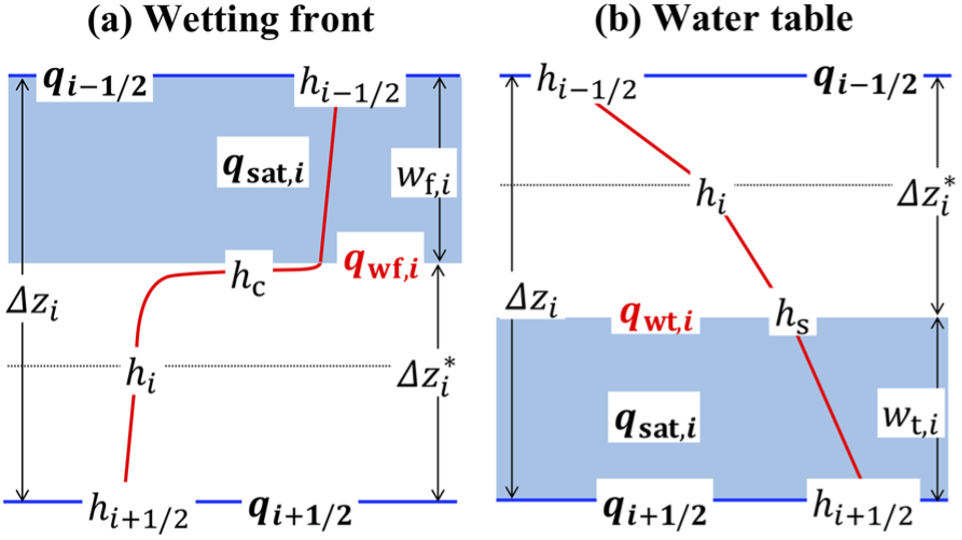
\includegraphics{Figures/陆地表面的水分循环/饱和-非饱和过渡状态的土壤层.png}
\caption{饱和-非饱和过渡状态的土壤层。如果土壤层内上部有饱和区(左图),
层内饱和区的厚度作为预报变量被激活;如果土壤层内下部有饱和区(右图),层内饱和区的厚度作为预报变量被激活。}
\label{fig:饱和-非饱和过渡状态的土壤层}
\end{figure}
}


预报变量($\theta_i$)的预报方程为
\begin{equation}\label{si_in1}
\left(\Delta z_{i}-w_{f, i}^{n+1}-w_{t, i}^{n+1}\right) \cdot\left(\theta_{i}^{n+1}-\theta_{i}^{n}\right)=\Delta t \cdot\left(q_{ {uin,i }}^{n+1}-q_{ {out }, i}^{n+1}\right)
\end{equation}
其中,$\Delta z_i$ 为第$ i $层土壤的厚度,$\Delta t$ 为时间步长,$q_{uin,i}^{n+1}$为非饱和区域上边界处的水流通量,$q_{out,i}^{n+1}$为非饱和区域下边界处的水流通量。


预报变量($w_{f,i}$)表示土壤层上部饱和区域的厚度,其预报方程为
\begin{equation}\label{si_in2}
\left(\theta_{s, i}-\theta_{i}^{n}\right) \cdot\left(w_{f, i}^{n+1}-w_{f, i}^{n}\right)=\Delta t \cdot\left(q_{i-1/2}^{n+1}-q_{w f, i}^{n+1}\right)
\end{equation}
其中,$\theta_{s,i}$ 为第$ i$ 层土壤的饱和体积含水量,$ q_{{i-1/2}}^{n+1}$为第$i$层土壤上边界处的水流通量,$q_{wf,i}^{n+1}$为饱和区域下边界处的水流通量。


预报变量($w_{t,i}$)表示土壤层下部饱和区域的厚度,其预报方程为
\begin{equation}\label{si_in3}
\left(\theta_{s, i}-\theta_{i}^{n}\right) \cdot\left(w_{t, i}^{n+1}-w_{t, i}^{n}\right)=\Delta t \cdot\left(q_{w t, i}^{n+1}-q_{i+1 / 2}^{n+1}\right)
\end{equation}
其中,$q_{wt,i}^{n+1}$  为饱和区域上边界处的水流通量,$q_{i+1/2}^{n+1}$为第$i$层土壤下边界处的水流通量。


在未饱和的土壤层,模式使用预报方程(\ref{si_in1})预报体积含水量的变化;
若未饱和的土壤层内上部有饱和区域,模式联合预报方程(\ref{si_in1})和(\ref{si_in2})来同时预报饱和区域的边界变化和非饱和区域内土壤积水含水量的变化;
若未饱和的土壤层内下部有饱和区域,模式联合预报方程(\ref{si_in1})和(\ref{si_in3})来同时预报饱和区域的边界变化和非饱和区域内土壤积水含水量的变化;
若未饱和的土壤层内上下部分均有饱和区域,模式联合预报方程(\ref{si_in1})--(\ref{si_in3})来同时预报饱和区域的边界变化和非饱和区域内土壤积水含水量的变化。


在地下部分,所有未饱和土壤层内的上述预报方程联合在一起组成一个方程组,来进行统一求解。

\subsection{地表积水的变化}
为了预报由入渗所产生的地表水深的变化,地表积水深度($h_{pond}$)也是算法中的预报变量,其预报方程为
\begin{equation}\label{hpond}
h_{ {pond }}^{n+1}-h_{ {pond }}^{n}=\Delta t \cdot\left(q_{ {surf }}^{n+1}-q_{ {infl }}^{n+1}\right)
\end{equation}
其中,$q_{surf}^{n+1} $ 为从地表水上部进入的水流通量,
其可以是降水、蒸发、或者地表水与积雪的液态水交换,$q_{infl}^{n+1}$为从地表进入土壤的水流通量。


当地表有积水,或者由于进入地表的水流通量大于入渗到土壤中的通量而形成积水时,积水深度的预报方程(\ref{hpond})也加入到土壤水的方程组中,进行统一求解。


\subsection{地下水的变化}
当地下水位在土壤水计算区域内部时,其位置由$w_{(t,i)}$进行预报。


当地下水位处于土壤水计算区域之下时,使用预报变量$W_a$来表示计算区域之下蓄水层的蓄水状态。$W_a$定义为
\begin{equation}
W_{a}=-\int_{z_{b t m}}^{Z_{w t}}\left(\theta_{s}-\theta\right) d z
\end{equation}
$W_a$的绝对值为土壤水计算区域之下单位面积上未填充液态水的孔隙的体积,
负号代表计算区域之下液态水是亏缺的。$W_a$的最大值为0,表示地下水位位于计算区域的下边界之上。


$W_a$的预报方程为
\begin{equation}\label{wa_n1_n}
W_{a}^{n+1}-W_{a}^{n}=\Delta t \cdot q_{b t m}^{n+1}
\end{equation}
当地下水位处于土壤水计算区域之下时,$W_a$的预报方程(\ref{wa_n1_n})也加入到土壤水的方程组中,进行统一求解。

\subsection{水流通量的计算}
预报方程(\ref{si_in1})--(\ref{wa_n1_n})中,右端项中均包含了水流通量的计算,其计算分为以下几种情形,
\begin{enumerate}
    \item 饱和区域内部的水流通量,使用公式
    \begin{equation}\label{q_sat1}
        q_{sat}=-\frac{\sum_{i=i_{1}}^{i_{2}} \Delta z_{i}}{\sum_{i=i_{1}}^{i_{2}} \frac{\Delta z_{i}}{K_{s, i}}}
         \cdot \frac{h_{l}-h_{u}-\sum_{i=i_{1}}^{i_{2}} \Delta z_{i}}{\sum_{i=i_{1}}^{i_{2}} \Delta z_{i}}
        \end{equation}
        其中,$i_1,i_1+1,…,i_2$为从上至下连续的饱和土壤层的层号,$\Delta z_i$为第i层的厚度,
        $K_{s,i}$为第$i$层的饱和土壤导水率,$h_l$为饱和区域下边界处的土壤水势。
        当饱和区域上边界为地表时,$h_u$取为地表积水深度$h_{pond}$;
        当饱和区域上边界在土壤内部时,$h_u$为饱和区域上边界处的土壤水势。
        (\ref{q_sat1})右端第一个分式计算了饱和区域的等效导水率,第二个分式计算了总水势的差商。

    \item 两个异质不饱和土壤层之间的水流通量,使用公式
    \begin{equation}\label{qht1}
        q_{h t}=q_{h m}\left(z_{i}-z_{u}, h_{u}, h_{i}\right)=q_{h m}\left(z_{l}-z_{i}, h_{i}, h_{l}\right)
        \end{equation}
        其中,$q_{ht}$为两层土壤间的水流通量,$z_u$为上层土壤的中心点的位置,$z_l$为下层土壤的中心点的位置,
        $z_i$为异质土壤的交界面的位置,$h_u$为$z_u$处的土壤水势,$h_l$为$z_l$处的土壤水势,$h_i$为$z_i$处的土壤水势。
        $q_{hm}$为计算均质土壤内水流通量的函数,它依赖于土壤层的厚度和上下边界处的土壤水势,
        (\ref{qht1})的含义为土壤层界面处的水流通量等于界面上方均质土壤内的水流通量,也等于界面下方均质土壤内的水流通量。
        土壤交界面处的土壤水势$h_i$为未知量,通过(\ref{qht1})的隐式方程进行求解后,再代入到(\ref{qht1})中计算$q_{ht}$. 函数$q_{hm}$为
        \begin{equation}
        q_{h m}\left(\Delta z, h_{u}, h_{l}\right)=-k_{h m} \cdot\left(\frac{h_{l}-h_{u}}{\Delta z}-1\right)
        \end{equation}
        其中,$\Delta z$为土壤层的厚度,$h_u$,$h_l$分别为土壤层上下两个边界处的土壤水势;
        $k_{hm}$为等效水力导度,其计算公式分为三种情况,对入渗情形($h_u>h_l$),
        \begin{equation}
        k_{h m}=\frac{1}{1-\frac{h_{l}-h_{u}}{\Delta z}} \cdot\left[k_{u}+\frac{h_{u}-h_{l}}{\Delta z}\left(k_{u}\right)^{1-r_{0}} \cdot\left(k_{l}\right)^{r_{0}}\right]
        \end{equation}
        对排水情形($h_l-\Delta z<h_u<h_l$),
        \begin{equation}
        k_{h m}=\left(k_{u}\right)^{r} \cdot\left(k_{l}\right)^{1-r}, r=\max \left(1+r_{0} \cdot \frac{h_{l}}{\Delta z}, 1-r_{0}\right)
        \end{equation}
        对毛细上升情形($h_u<h_l-\Delta z$),
        \begin{equation}
        k_{h m}=\left(k_{u}\right)^{r_{0}} \cdot\left(k\left(h_{l}-\Delta z\right)\right)^{1-r_{0}}
        \end{equation}
        其中,土壤水力导度$k$为土壤水势$h$的函数,上述三个公式中,$k_u=k(h_u )$,$k_l=k(h_l )$;
        $r_0$是依赖于土壤水力模型和土壤水力参数的参数,对Campbell模型,
        \begin{equation}
        r_{0}=\frac{1}{3 \lambda+2}
        \end{equation}
        对van Genuchten--Mualem模型,
        \begin{equation}
        r_{0}=\frac{1}{L(n-1)+2 n}
        \end{equation}
        预报方程(\ref{si_in1})--(\ref{si_in3})为隐式时间积分格式,上述水流通量的计算公式可在理论上保证在均质土壤中,
        预报方程(\ref{si_in1})--(\ref{si_in3})的解为本质无振荡的,也可在土壤具有分层异质性时,提高计算的稳定性和精度。

    \item 饱和区位于非饱和区上方时两者之间的水流通量,公式为
    \begin{equation}
    q_{w f}=q_{h m}\left(z_{l}-z_{i}, h_{s}, h_{l}\right)
    \end{equation}
    其中,$z_u$为上方非饱和土壤层中心点的位置,$z_i$为饱和区和非饱和区之间界面的位置,
    $h_s$为饱和土壤水势,$h_u$为非饱和土壤层中心点处的土壤水势。
\end{enumerate}


\subsection{预报方程的求解}
预报方程(\ref{si_in1})--(\ref{hpond})和(\ref{wa_n1_n})的左边均代表水量的变化,右边均代表土壤层边界上的水流通量,若在某时刻,
活动预报变量的个数为$A$,则可将第$\alpha$个变量对应的方程表达为
\begin{equation}\label{m_alpha_x}
\delta m_{\alpha}(\vec{x})=\Delta t \cdot \delta q_{\alpha}(\vec{x})
\end{equation}
其中$\vec{x}$⃗代表活动预报变量组成的向量,由(\ref{m_alpha_x})可得带约束的非线性最小二乘问题
\begin{equation}
\begin{aligned}
\min _{\vec{x}} f_{2}(\vec{x})=& \min _{\vec{x}} \sum_{\alpha=1}^{A}\left(\delta m_{\alpha}(\vec{x})-\Delta t \cdot \delta q_{\alpha}(\vec{x})\right)^{2} \\ 
& \theta_{r, i}<\theta_{i} \leq \theta_{s, i}, & \forall \theta_{i} \in \vec{x} \\ 
& 0 \leq w_{f, i} \leq \Delta z_{i},               & \forall w_{f, i} \in \vec{x} \\ 
& 0 \leq w_{t, i} \leq \Delta z_{i},               & \forall w_{t, i} \in \vec{x} \\ 
& h_{ {pond }} \geq 0,                               & \text{ if } h_{ {pond }} \in \vec{x} 
\end{aligned}
\end{equation}
此问题采用Gauss--Newton迭代算法进行求解。